\documentclass[12pt,]{article}
\usepackage{beamerarticle}
\usepackage[utf8]{inputenc}
\usepackage{hyperref}

% Math
\usepackage{amssymb,amsmath,amsthm} 
\newtheorem{proposition}{Proposition}

% Fontfamily
\usepackage{palatino}%\usepackage{lmodern, times}

% Page settings
\usepackage[letterpaper, margin=1in]{geometry}
\usepackage{setspace}                           
\onehalfspacing %\doublespacing  % \singlespacing 

% Appendix
\usepackage{appendix}

% Line numbers
%\usepackage{lineno}
%\linenumbers


% Tables
\usepackage{array,booktabs,longtable,rotating}
\newenvironment{tablenotes}[1][]{
  \begin{minipage}{\textwidth}\emph{Notes:}{\footnotesize #1}
}{\end{minipage}}
\makeatletter
\def\fps@table{htbp}
\makeatother

% Graphics
\usepackage{graphicx,grffile}
\makeatletter
\def\maxwidth{\ifdim\Gin@nat@width>\linewidth\linewidth\else\Gin@nat@width\fi}
\def\maxheight{\ifdim\Gin@nat@height>\textheight\textheight\else\Gin@nat@height\fi}
\makeatother
% Scale images if necessary, so that they will not overflow the page
% margins by default, and it is still possible to overwrite the defaults
% using explicit options in \includegraphics[width, height, ...]{}
\setkeys{Gin}{width=\maxwidth,height=\maxheight,keepaspectratio}
% set default figure placement to htbp
\makeatletter
\def\fps@figure{htbp}
\makeatother

\usepackage{natbib}% plainnat
\bibliographystyle{aer}


\setlength{\emergencystretch}{3em}  % prevent overfull lines
\providecommand{\tightlist}{%
  \setlength{\itemsep}{0pt}\setlength{\parskip}{0pt}}



\title{Races or Tournaments?\thanks{Blasco: Harvard Institute for Quantitative Social Science, Harvard
University, 1737 Cambridge Street, Cambridge, MA 02138 (email:
\href{mailto:ablasco@fas.harvard.edu}{\nolinkurl{ablasco@fas.harvard.edu}}).}}
\author{Andrea Blasco \and Kevin J. Boudreau \and Karim R. Lakhani \and Michael Menietti}
\date{Last updated: 18 January, 2017}

\begin{document}
\maketitle
\begin{abstract}
A wide range of economic and social situations are decided by either a
race or a tournament. In either situations, agents choose whether and
how much to exert some costly effort to increase the probability of
being awarded a prize under the uncertainty about the actions of other
agents. While a tournament yield outcomes greater than those of a race,
the latter prevents unnecessary costs due to an excess of participation.
We examine this trade-off empirically. We report the results of a field
experiment conducted online where we compare the outcomes --- efforts,
quality, and diversity of outputs --- of three alternative competitive
situations motivated by theory: the race, the tournament, and the
tournament with a quality requirement.

\smallskip\noindent 
JEL Classification: xxx; xxx; xxx.

\smallskip\noindent 
Keywords: xxxx; xxxx xxxx.
\end{abstract}


% Todo notes
%\usepackage[textsize=tiny]{todonotes}
%\newcommand\redmarginpar[1]{\marginpar{\footnotesize{\textcolor{red}{#1}}}}
%\listoftodos[Notes]
\clearpage
\tableofcontents
\setcounter{tocdepth}{2}
\clearpage

\section{Introduction}\label{introduction}

Contests are a very important source of incentives in the economy. In
the United States, the government regularly sponsors open competitions
aimed at solving challenging problems on a variety of important issues
including public health, education, energy, and environment protection.
Increasingly, contests are conducted online in the spirt of open
innovation initiatives as in xxxx, xxxx, xxxx. For example, the web
portal www.challenge.gov regularly hosts online challenges to engage a
worldwide population of potential problem-solvers in xxxx. In the
private sector, firms use contests as an effective tool to expand its
innovative capacity or, internally, in the form of bonuses or promotion
mechanisms leading workers to exert higher levels of effort.

Greeks.

In this study, we focus on the difference between two quite popular
choices of contest design: the ``race'' (a competition to be first) and
the ``tournament'' (a competition to be best). In particular, we aim at
addressing the following research questions: How this choice affect the
choices of contestants? When the sponsor of a competition should pick
one or the other? What is the main trade-off? How this decision interact
with other key choices of design such as the distribution of prizes
among winners?

To address these questions we proceed in two ways. First, we generalize
the well known incomplete information contest model of
\citet{moldovanu2001optimal}. This is enables a direct comparison of
equlibrium behaviors under both the race and the tournament within a
single theoretical framework. Then, we collect data from a field
experiment that we desiged and run to test some of the implications of
the theory, and provide policy recommendations.

The design of a contest has received much attention among economists.
Economists have a long tradition in studying races of various kinds
(patent and arms races), and tournaments (sales tournaments). A large
body of works have investigated several aspects of contest design,
including the optimal prize structure {[}XXX{]}, number of competitors
{[}XXX{]}, and the appeal of imposing minimum effort requirments
{[}XXX{]}. Seldom economists have considered the competitive setting
being either a race or a tournament as the result of a deliberate choice
of contest design. Usually the nature of the competition is seen as
exogenous and due to the environemental factors (for example, in a
patent race, the type of competition is determined by the legal
environment and cannot be easily changed by policy makers). One
important exception is \citet{baye2003strategic} that identifies a
strategic equivalence between games of complete information modeled as
races and tournaments. This paper is important because connects extends
to races the results from a wide literature on the optimal design of a
tournament. However, it does not shed light on when it would be
desirable to use one or the other.

By this perspective, we are able to show that races cannot be justified
simply by the goal of maximizing average effort. And the reason is
intuitive. A race awards a prize to first to hit a particular target.
Those who will judge the target to hard to achieve will not join the
competition and will drop out. On the contrary, those who are able to
achieve the target at low costs will not try to exceed the target. As a
result, the race is comparable to a competition with fixed ``entry
costs'' or a fixed entry requirement, where agents will decide to either
enter and pay a fixed prize, or stay out of the competition. Then, the
possible gains in terms of expected revenues from a race are limited to
those who would enter the competition and would exert less effort that
that required to hit the target. These potential benefits can be
obtained under a tournament as well by imposing a a fixed requirement to
be eligible for prizes. So, races are not chosen to maximize expected
effort of competitors, at least, in the traditional
``auction-theoretical'' sense.

What are races for? We examine a few hypothesis and we provide some
examples. First hypothesis is that the sponsor of the race is not
primarily interested in total output but also in the time to complete a
particular task. In a tournament, this type of preferences can be
satisfied by fixing a deadline. Say time within which competitors are
asked to provide their efforts. However, assuming competitors have costs
from making less time in performing a task and there complementarities
in costs, increasing the deadline in a tournament is similar to raising
the marginal cost for everyone, which might not be an optimal solution.
In a race, by contrast, increasing the deadline will affect entry but,
conditional on entry, the time to complete the task will always be less
than the deadline. Which means that those with low costs will be mostly
affected by the deadline, whereas xxxx. Which may be a superior choice
than the tournament.

To fix ideas let consider the following example. The government wants to
solve a global public health problem such as ``antibiotics resistance.''
The overuse of antibiotics leads to the phenomenon of ``resistance''
which is a loss in the power of antibiotics to treat certain infections.
This is an increasing threat for public health. The government has the
choice of making a contest to engage people in solving this problem. The
government has preferences for time in the sense that the government
wants to minimize to have the first submission. So, the government fix a
requirement in terms of costs of the solution and award a prize to the
first to meet this requirement. Example. UK governemet goes for a race.
EU xxxx goes for a tournament with a deadline in 2016. (\ldots{}) The
answer to this optimal design question relates to the cost function of
agents with respect to ``time'' and to ``effort.'' It is hard to say
which solution is better. However, it is easier to tell whether you
should have one prize or multiple prizes.

There is also a case for efficiency. Consider a platform with many
competitions. The platform may want to engage competitors for short
period of time provide that solutions are above a certain quality level.

To test our theory we further examine experimental data on competitors
making sumibssion in an online computer programming contest. We
randomized competitors into 3 groups: 1. race 2. tournament 3.
tournament with a quality requirement we study participation, timing of
submission and final scores.

We find that, as our theory suggest, participation is higher in the
tournament and lower in the race and in the tournament with entry costs.
We further find that submission are quicker in a race, whereas are
equally distributed at the end of the competition in the the tournament
and in the tournament with quality requirement. With respect to final
scores, theory predicts as trade-off between a race and a tournament in
terms of higher scores vs faster submissions. We do find that scores are
higher in the tournament but we do not find a strong trade-off in the
sense that race had comparable good quality solutions than the
tournament.

\section{Literature}\label{literature}

This paper is related to the contest theory literature
\citet{dixit1987strategic} \citet{baye2003strategic},
\citet{parreiras2010contests}, \citet{moldovanu2001optimal},
\citet{moldovanu2006contest}, \citet{siegel2009all},
\citet{siegel2014contests}. It also relates to the literature on
innovation contests \citet{taylor1995digging}, \citet{che2003optimal}.
And the personnel economics approach to contests \citet{lazear1981rank},
\citet{green1983comparison}, \citet{mary1984economic}.

Empirically, \citet{dechenaux2014survey} provide a comprehensive summary
of the experimental literature on contests and tourments. Large body of
empirical works have focused on sports contests
\citet{szymanski2003economic}. More recently, inside firms (xxx) and
online contest (xxxx).

This paper is also related to the econometrics of auctions
\citet{paarsch1992deciding}, \citet{laffont1995econometrics},
\citet{donald1996identification} and more recently
\citet{athey2011comparing}, \citet{athey2002identification}, and
\citet{athey2007nonparametric}.

\section{The model}\label{the-model}

def: A contest is a N player game. Players move simultaneously and
select a performance variable \(y_i\) (the xxxx in performing a task)
and a timing \(t_i\) (to complete a task), both being nonnegative
numbers. Players are ranked according to their choices and a player's
rank is given by the function \(r_i(y_1,...y_N, t_1, ..., t_N)\). The
top \(K\) ranked players (e.g., \(r_i<K\)) are awarded a prize of value
\(V_1 > V_2 > ... > V_K\).

The goal for each player is to maximize the expected utility. If the
timing is above a given deadline \(d>0\) or the performance is below a
certain level \(q>0\), the player gets zero utility. Otherwise, the
player is given a rank based on his performance and timing. A contest is
xxxx. Ranked .

def: A tournament is a xxxx where players are ranked by their
performance level provided that the timing is below a deadline \(d\).

def: A race is a xxxx where players are ranked by their timing provided
that the performance is above a threshold level \(q\).

In a tournament, the agent having achieved the highest output quality
within the deadline gets the first prize, the agent having achieved the
second highest output quality gets the second prize, and so on. In a
race, by contrast, the first agent to achieve an output quality of at
least \({\bar y}\) within the deadline wins the first prize, the second
to achieve the same target gets the second prize, and so on.

Since agents move simultaneously, they do not know the performance of
others when deciding their efforts. On the other hand, it is assumed
that they know the number of competitors as well as their cost functions
to complete the task up to a factor \(a_i\) being the agent's private
ability in performing the task. Each agent knows his ability but does
not know the ability of the others. However, it is common knowledge that
abilities are drawn at random from a common distribution \(F_A\) that is
assumed everywhere differentiable on the support
\(V\subseteq [0, \infty)\).

It is further assumed that costs are multiplicative

\[C(y_i, t_i, a_i) = {c_{y}}(y) \cdot {c_{t}}(t)  \cdot a_i^{-1}\]

with \({c_{y}}(0)\geq 0\), \({c_{y}}^\prime>0\), \({c_{t}}(d)\geq 0\),
and \({c_{t}}^\prime<0\).

Each agent is risk neutral and faces the following decision problem

\[\begin{array}{ll}
    \mbox{maximize} & \sum_{j=1}^k \Pr(\text{ranked $j$'th}) V_j  - C(y_i, t_i, a_i).
  \end{array}\]

\subsubsection{Equilibrium in a
tournament}\label{equilibrium-in-a-tournament}

We provide here the symmetric equilibrium with one prize and \(n>2\)
agents. In appendix XXX, we provide a general formula for \(k>2\)
prizes.

Let \(y_{1:n} < y_{2:n} < ... < y_{n:n}\) denote the order statistics of
the \(y_j\)'s for every \(j\neq i\) and let \({F_{Y_{r:n}}}(\cdot)\) and
\({f_{Y_{r:n}}}(\cdot)\) denote the corresponding distribution and
density for the \(r\)'th order statistic.

\begin{proposition}

In a tournament, the unique symmetric equilibrium of the model gives,
for every \(i=1, ..., n\), the optimal time to completion \(t^*(a_i)\)
equal to the deadline \(d\) and the optimal output quality \(y^*(a_i)\)
as

\[\label{eq: optimal bid tournament}
  y^*(a_i) =  V_1 \int_{a_i}^\infty {f_{Y_{n:n}}} (z) dz\]

if \({a_i}\geq {\underline a}\) \citep[see][]{moldovanu2001optimal}, and
equal to zero otherwise.

\end{proposition}

An important property of is that \(y^*(a_i)\) has its upper bound in and
lower bound in . Also, equilibrium output quality is monotonic
increasing in the agent's ability \citep[see][]{moldovanu2001optimal}.
Thus, for every \(i=1, ..., n+1\), the equilibrium expected reward
depends only on the rank of his ability relative to the others. Using
\({F_{A_{r:n}}}\) to denote the distribution of the \(r\)'th order
statistic of abilities gives

\[\label{eq: expected payoffs tournament}
  {F_{A_{n:n}}}(a_i) V_1  - C(y_i^*, d, a_i).\]

Hence, by setting to zero and solving for the ability, gives the
marginal ability \({\underline a}\) as

\[{\underline a}= h(n, V, F_A, C, d).\]

\begin{corollary}

Equilibrium behavior in a race

\end{corollary}

\subsubsection{The expected revenues for the sponsor of the
contest}\label{the-expected-revenues-for-the-sponsor-of-the-contest}

The sponsor of the contest chooses the rules of the competition
including prize structure \(\{V_j\}_{j=1}^k\), deadline \(d\), target
quality \(q\), and competition format (race or tournament). The sponsor
maximizes an objective function that is the sum of total quality
\(Y=\sum_{i=1}^{n+1} Y_i\), time spent \(T=\sum_{i=1}^{n+1} T_i\) and
prizes paid \(V=\sum_{j=1}^k p_{j} V_j\) (with \(p_j=1\) if the prize is
awarded and \(p_j=0\) otherwise). Hence, the problem faced by the
sponsor is

\[\begin{array}{ll}
    \mbox{maximize} & \int {Y}   -  {\tau}{{\bf E}}{T} - {{\bf E}}{V}
  \end{array}\]

with the intensity of preferences towards time weighted by
\(c_t\geq 0\).

\subsection{Structural econometric
model}\label{structural-econometric-model}

\section{The field experiment}\label{the-field-experiment}

\subsection{The context and experimental
design}\label{the-context-and-experimental-design}

The field experiment was conducted in the context of an online
programming competition hosted on the platform Topcoder.com between
March 2 and 16, 2016. A programming competition generally involves
contestants writing source code to solve given problems. Since its
launch in 2001, Topcoder.com administers on a weekly basis several
competitive programming contests for thousands of competitors from all
over the world. Typical assigned problems are data science problems
(e.g., classification, prediction, natural language processing) that
demand some background in machine learning and statistics. All Topcoder
members (about 1M registered users in 2016) can compete and attain a
``rating'' that provides a metric of their ability as contestants. Other
than attaining a rating, the competitors having made the top five
submissions can be also awarded a monetary prize, the extent of which
range depends on the nature and complexity of the problem but is
generally between \$5,000 to \$20,000.

In this study, we worked together with researchers from the United
States National Health Institute (NIH) and the Scripps Research
Institute (SCRIPPS) to select a challenging problem for the experimental
programming competition. The selected problem was based on an algorithm,
called BANNER, built by NIH that uses expert labeling to annotate
abstracts from a prominent life sciences and biomedical search engine,
PubMed, so disease characteristics can be more easily identified
\citep[see][]{leaman2008banner}. The goal of the programming competition
was to improve upon the current NIH's system by using a combination of
expert and non-expert labeling, as described by
\citet{good2014microtask}.

The competition was announced on the platform and to all community
members via email. A preliminary registration was mandatory. A limit of
max 300 participants was established {[}Why?{]}. Only participants with
a positive rating were allowed to compete. Following a three days
registration period, signed up competitors were randomly assigned to
separate groups also called ``virtual rooms''. In each of these rooms,
contestants were given a list of competitors in the same room and a chat
to communicate with the platform managers and ask clarifying questions
about the problem. Everyone received the same computational problem, as
described above, and had to develop a solution within a period of 2
weeks.

These virtual rooms were then randomly assigned to one of three
different competitive settings: a race, a tournament, and a tournament
with a minimum quality requirement. Monetary payoffs were the same in
all groups: the first placed competitor was awarded a prize of \$1,000,
and an additional, consolatory prize of \$100 was awarded to the second
one. However, in a race, the first to xxxx. In a tournament, xxxx .And
in a tournament with minimum quality requirement, xxxx. Grand prizes of
xxxx were awarded to the top xxx in every treatment.

\subsection{Data}\label{data}

Individual data about each competitor were obtained from the online web
profile on the platform. This profile typically includes when the member
registered to the platform, the current rating, the number of past
competitions, and so on. Additional personal information, was collected
via a mandatory initial and a final survey. In the initial survey,
registered competitors were asked basic demographics, including a
measure of risk aversion. They were also asked to forecast the number of
hours they would be able to spend competing in the next few days (the
exact question was: ``looking ahead xxxx''). In the final survey, they
were asked to look back and tell us their best estimate of the time
spent working on the problem.

A total of xxxx registered but only 299 competitors were selected for
the challenge; we excluded those with no past experience on the platform
and those with incomplete data on the survey. Signed up competitors were
experienced members of the platform: the overall time as registered
platform member at the start of the competition ranged between 52.571
and 770.571 weeks. Yet, the direct experience in competing was highly
skewed with competitors in the highest 90th percentile having
participated in 28.2 more competitions than those in the 10th
percentile. Likewise skills as measured by the individual ratings, if
there was one, had a skewed distribution with 999 higher points than
those in the 10th percentile; see Figure
\ref{eq: distribution experience}.

After the two-week submission period, 86 competitors made 1759
submissions overall. The distribution of submissions was rather skewed,
with participants in the 90th percentile making 50 more submissions than
those in the 10th percentile.

Assuming the decision was independent, to explore the determinants of
participation:

\begin{equation}
  Pr(y=1) = G(\text{Rating}_{i} + \text{Experience}_{i} + \text{T}_{i})
\end{equation}

where \(G()\) is logistic.

\begin{verbatim}
## Analysis of Deviance Table
## 
## Model: binomial, link: logit
## 
## Response: nsub > 0
## 
## Terms added sequentially (first to last)
## 
## 
##                           Df Deviance Resid. Df Resid. Dev Pr(>Chi)
## NULL                                        298        359         
## poly(mm.count, deg = 2)    2    21.97       296        337  1.7e-05
## poly(mm.rating2, deg = 2)  2    11.86       294        325   0.0027
## poly(msince2, deg = 3)     3     2.36       291        323   0.5011
## poly(mm.top10, deg = 2)    2     3.93       289        319   0.1405
## poly(badges, deg = 2)      2     1.47       287        317   0.4785
\end{verbatim}

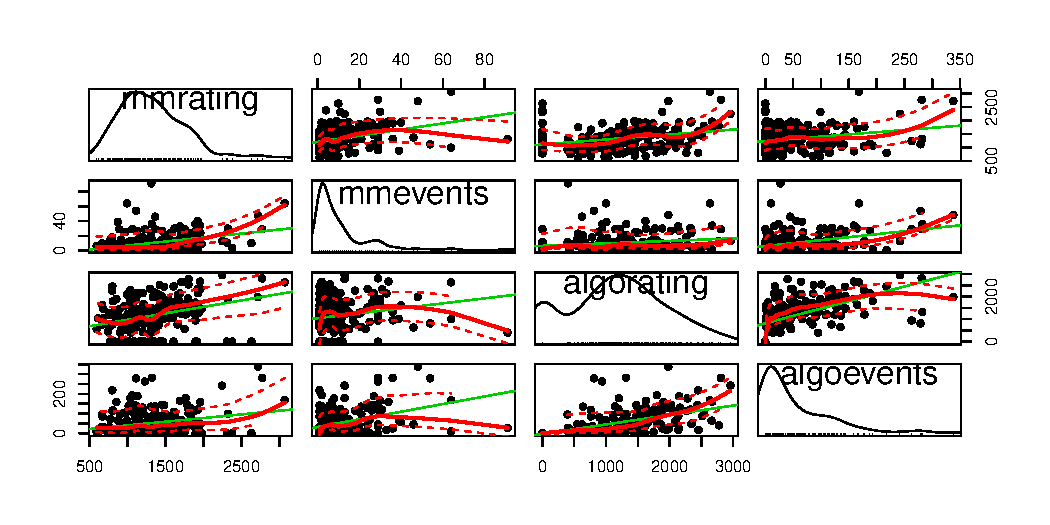
\includegraphics{Figures/unnamed-chunk-8-1.pdf}

This result does not seem to correlate well with the competitor's
experience or skills, as the Pearsons's correlation coefficient between
the count of past competitions or the rating and the count of
submissions is positive but generally low; see Table XXX. Thus,
differences in submissions appear idiosyncratic and perhaps related to
the way to organize the work rather than systematically associated with
underlying differences in experience or skills.

\begin{verbatim}
##            nsub mm.rating mm.count
## nsub      1.000     0.181    0.178
## mm.rating 0.181     1.000    0.333
## mm.count  0.178     0.333    1.000
\end{verbatim}

The timing of submissions was rather uniform during the submission
period with a peak of submissions made in the last of the competition.
(explain more)

\begin{verbatim}
scores$submax <- ave(scores$subid, scores$id, FUN=max)
par(mfrow=c(2, 1), mar=c(4,4,2,2))
plot(subid==1 ~ as.POSIXct(subts), data=scores, type='h', yaxt='n'
    , xlab='', ylab='', main='Dispersion time first submission')
plot(subid==submax ~ as.POSIXct(subts), data=scores, type='h'
    , yaxt='n', xlab='', ylab='', main='Dispersion time last submission')
\end{verbatim}

Scores: xxxx

\section{Empirical analysis}\label{empirical-analysis}

\subsection{Treatment differences}\label{treatment-differences}

Difference in participation by treatments are show in Table XX.

We find no differences in the room size.

Ex-post

\begin{verbatim}
## Warning in bxp(structure(list(stats = structure(c(784858.58, 794084.93, :
## some notches went outside hinges ('box'): maybe set notch=FALSE
\end{verbatim}

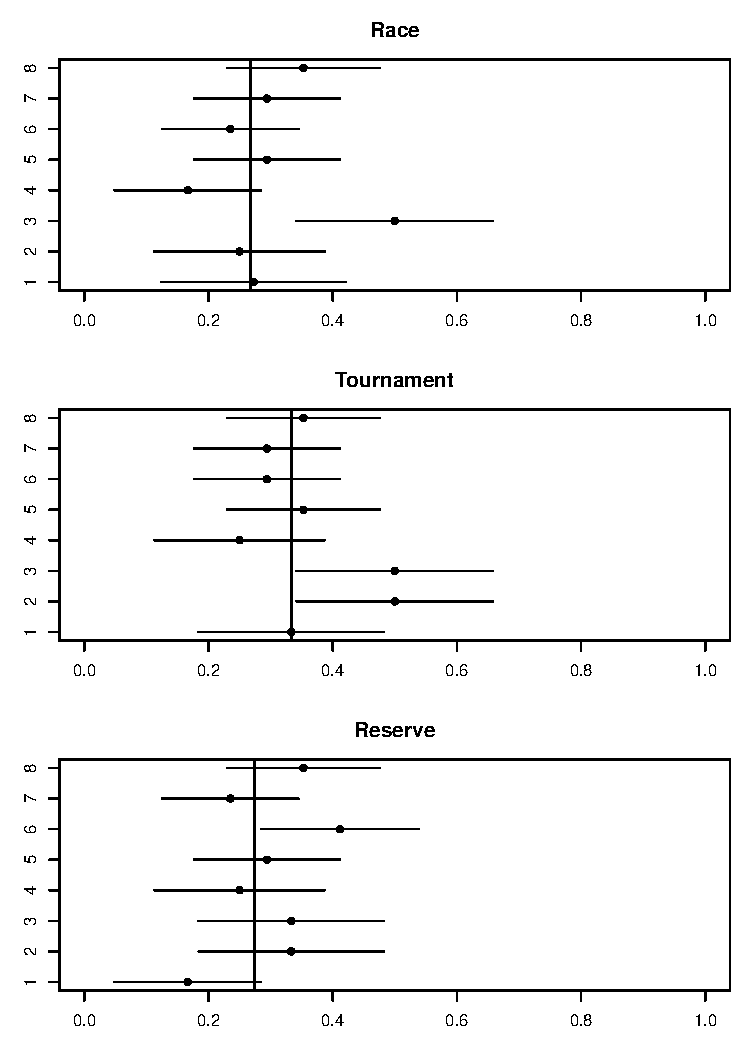
\includegraphics{Figures/unnamed-chunk-12-1.pdf}
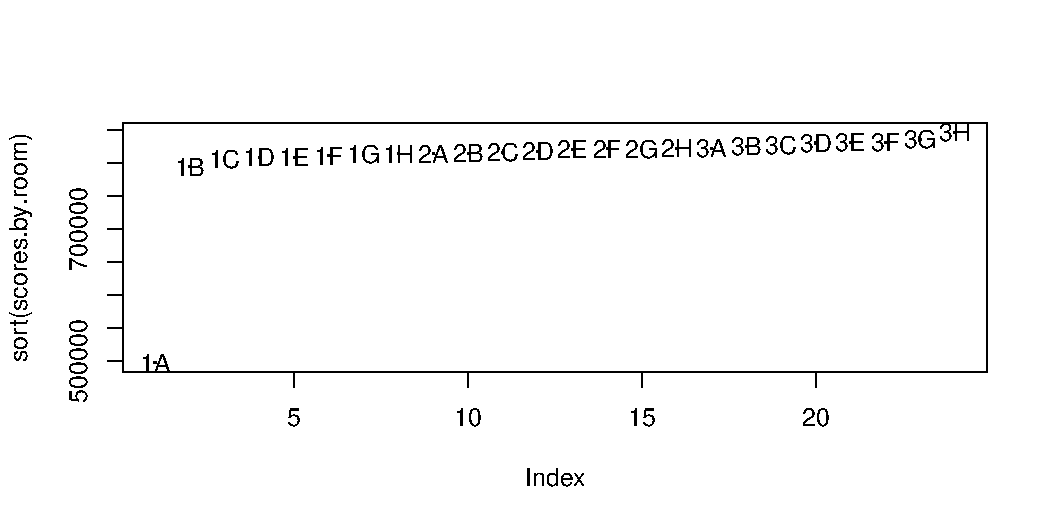
\includegraphics{Figures/unnamed-chunk-12-2.pdf}

Timing: early vs late

Using a Chi-square test of independence, we find no significant
differences in participation rates associated with the assigned
treatments (p-value: 0.000419); see Table XX.

Further, we model participation rates as a logistic regression. We use a
polynomial of third degree for the count of past competitions to account
for non-linear effects of experience; and we use an indicator for
whether the competitor had a win or not. Also, taking into account
differences in ability, participation rates are not significantly
different.

\subsection{Estimation results}\label{estimation-results}

Participation to the competition by treatment is shown in Figure
\ref{fig:entry}. Participation here is measured by the proportion of
registered participants per treatment who made any submission during the
eight-day submission period. Recall that competitors may decide to enter
into the competition and work on the problem without necessarily
submitting. In a tournament, for example, competitors are awarded a
prize based on their last submission and may decide to drop out without
submitting anything. However, this scenario seems unlikely. In fact,
competitors often end up making multiple submissions because by doing so
they obtain intermediate feedback via preliminary scoring (see Section
XXX for details). In a race, competitors have even stronger incentives
to make early submissions as any submission that hits the target first
wins.

\begin{verbatim}
Table xxx
\end{verbatim}

We find that the propensity to make a submission is higher in the
Tournament than in the Race and in the Tournament with reserve, but the
difference is not statistically significant (a Fisher's exact test gives
a p-value of \texttt{round(fisher.test(nsub.tab)\$p.val,3)}). As
discussed in Section XXX, we may not have enough power to detect
differences below 5 percentage points. However, we find the same
not-significant result in a parametric regression analysis of treatment
differences with controls for the demographics and past experience on
the platform; see Table \ref{entry}. Adding individual covariates
reduces variability of outcomes, potentially increasing the power of our
test. In particular, Table \ref{entry} reports the results from a
logistic regression on the probability of making a submissions. Column 1
reports the results from a baseline model with only treatment dummies.
Column 2 adds demographics controls, such as the age, education, and
gender. Column 3 adds controls for the past experience on the platform.
Across all these specifications, the impact of the treatment dummies
(including room size) on entry is not statistically significant.

\subsection{Simulation results}\label{simulation-results}

\section{Empirical analysis}\label{empirical-analysis-1}

\subsection{Estimation results}\label{estimation-results-1}

Participation to the competition by treatment is shown in Figure
\[fig:entry\]. Participation here is measured by the proportion of
registered participants per treatment who made any submission during the
eight-day submission period. Recall that competitors may decide to enter
into the competition and work on the problem without necessarily
submitting. In a tournament, for example, competitors are awarded a
prize based on their last submission and may decide to drop out without
submitting anything. However, this scenario seems unlikely. In fact,
competitors often end up making multiple submissions because by doing so
they obtain intermediate feedback via preliminary scoring (see Section
XXX for details). In a race, competitors have even stronger incentives
to make early submissions as any submission that hits the target first
wins.

\begin{verbatim}
Table xxx
\end{verbatim}

We find that the propensity to make a submission is higher in the
Tournament than in the Race and in the Tournament with reserve, but the
difference is not statistically significant (a Fisher's exact test gives
a p-value of \texttt{r~round(fisher.test(nsub.tab)\$p.val,3)}). As
discussed in Section XXX, we may not have enough power to detect
differences below 5 percentage points. However, we find the same
not-significant result in a parametric regression analysis of treatment
differences with controls for the demographics and past experience on
the platform; see Table \[entry\]. Adding individual covariates reduces
variability of outcomes, potentially increasing the power of our test.
In particular, Table \[entry\] reports the results from a logistic
regression on the probability of making a submissions. Column 1 reports
the results from a baseline model with only treatment dummies. Column 2
adds demographics controls, such as the age, education, and gender.
Column 3 adds controls for the past experience on the platform. Across
all these specifications, the impact of the treatment dummies (including
room size) on entry is not statistically significant.

\subsection{Simulation results}\label{simulation-results-1}

\renewcommand\refname{References}
\bibliography{/Users/andrea/Papers/library.bib}

\end{document}